%%% KCSS Dissertation Template
%%%
%%% Take care of all fields marked <++FOO++>.
%%% When using Vim LaTeX Suite <http://vim-latex.sourceforge.net/>,
%%% then Ctrl-j should navigate to the next such field.

\documentclass[10pt]{book}
\usepackage[language=english,theorems=numbersfirst,paper=a4paper]{ifiseries}
\usepackage{listings}
\usepackage[ruled,vlined]{algorithm2e}
\usepackage{pdfpages}
\usepackage{todonotes}
\usepackage{breakurl}
\usepackage{subcaption}
\usepackage{hyperref}
\usepackage{lipsum}
\usepackage{parcolumns}
\setlength{\marginparwidth}{3cm}
\addbibresource{thesis.bib}

\graphicspath{{./assets/}}

\newenvironment{localsize}[1]
{%
  \clearpage
  \let\orignewcommand\newcommand
  \let\newcommand\renewcommand
  \makeatletter
  \input{bk#1.clo}%
  \makeatother
  \let\newcommand\orignewcommand
}
{%
  \clearpage
}

\newcommand{\figureref}[1]{\textbf{\autoref{#1}}}
\newcommand{\figurereft}[2]{\textbf{\autoref{#1} #2}}
\newcommand{\toxdo}[1]{}

\newcommand*\NewPage{\newpage\null\thispagestyle{empty}\newpage}

\begin{document}

\frontmatter

\studtitlepage%
{ArUco Marker Detection on Flexible Photonic Crystals}%
{}
{Niklas Carstensen}%
{Master's Thesis}%
{\today}%
{Prof. Dr. Reinhard Koch}%
{Jakob Nazarenus, Tim Michels}%
\NewPage{}
\setcounter{page}{2}
\studeidesstatt
\NewPage{}

\selectlanguage{english}
\setcounter{page}{3}
\chapter*{Abstract}
TODO

\tableofcontents
\listoffigures
%\listoftodos
\mainmatter
\chapter{Introduction}

The world faces a shortage of health workers, that is projected to endure into 2030 \cite{BMJHealthWorkforce22}, while 47\% of available health workers cared for 22\% of the worlds population in 2020. This shortage and unequal distribution of health workers drive the need for more efficient care for patients. 

A part of the solution for this problem could be small and inexpensive testing equipment \cite{Fab23}, which would allow for fast and regular assessment of ones health without requiring the time of healthcare professionals \cite{POC12}. Such an approach is called \ac{POC}, since the testing and evaluation is done by and of the patient. These kits are also called \acp{POCT}. One type of \ac{POCT} are wearables. However traditional wearables are based on electrical readout systems \cite{gao2019flexible}, which necessitate conducting wires, a battery and may be invasive. To overcome the drawbacks of wearables using electrical readout systems, optical readout systems can be used instead \cite{nguyen2021wearable}. One approach for an optical readout system is using commercially available adhesive tape, which acts as a \ac{PCS}, and etching \ac{ArUco} fiducial markers into it \cite{Fab23}. This is done by first applying a negative photoresist to the tape and then shining UV light on it, while masking the parts of it that are supposed to become part of the \ac{ArUco} shape later. Then an \ac{IBE} process is applied to the tape and finally the heat resist of the first step is removed during an ultrasonic heat bath.

\section{Problem Statement}

This work focuses on the detection of the \ac{ArUco} fiducial markers, that were etched into tape, using neural networks. Since the tapes should be used as \acp{POCT} by patients, the technology developed here is supposed to run on patients smart phones. While smart phones are easily carryable, they come with the drawback of not having much space or energy for large \acp{GPU}, which limits the choice of networks.

\section{Outline}

TODO

\chapter{Preliminaries}
\label{chap:prelim}

\section{Definitions}

The term dataset\footnote{\url{https://en.wikipedia.org/wiki/Data_set}, accessed at 01.10.2023} is central to machine learning as it defines what is learned from. However this term is ambiguous as it describes both a series of images and labels\footnote{\url{https://pytorch.org/tutorials/beginner/introyt/trainingyt.html}, accessed at 01.10.2023} as well as multiple groups of series of images and labels \cite{lin2014microsoft}. In other subfields of machine learning a dataset may contain different data types other than images. For this thesis however dataset and similar terms are defined as follows to make the later parts more easily understandable:

\begin{description}
  \item[Label] A \textit{label} or \textit{annotation} refers to extra data that belongs to an image and describes a subset of the images contents. \textit{Labels} are usually created using human input and describe the desired output of a machine learning model on that image.
  \item[Dataseries] A \textit{dataseries} refers to a series of images and labels
  \item[Dataset] A \textit{dataset} refers to a combination of usually up to three \textit{dataseries}.
  \item[Datagroup] A \textit{datagroup} refers to a \textit{dataseries} in the context of a \textit{dataset}. Typical \textit{datagroups} are 'training', 'validation' and 'testing' or 'train', 'val' and 'test' for short.
\end{description}

\section{Neural Networks}

This section gives a brief overview over \acp{ANN}. Since this thesis is written from a computer science perspective the term \acp{NN} is used interchangeably with \acp{ANN}.

\subsection{History}

Neural network interest and therefore research happened in waves over the last decades, starting with McCulloch and Pitts' work on logical operations on neurons in 1943 \cite{mcculloch1943logical,485891}. 

\begin{figure}
  \caption{Visualization of a perceptron}
  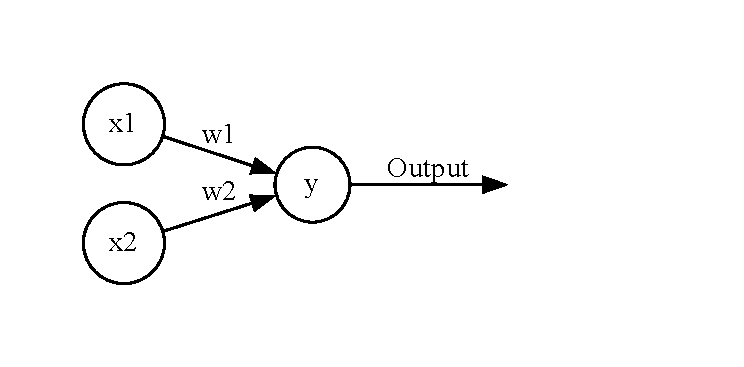
\includegraphics[width=0.5\textwidth]{graph/rosenblatt}
  \label{fig:perceptron}
\end{figure}

The second wave started in the early 1960ies with Rosenblatt's perceptron convergence theorem \cite{rosenblatt1962principles}. A visualization of the perceptron can be seen in \figureref{fig:perceptron} and the output of the perceptron is calculated as follows:
\[
    p(x)= 
\begin{cases}
    1, & \text{if } \sum_i w_ix_i + b > 0\\
    0, & \text{otherwise}
\end{cases}
\]
Setting $w1$ and $w2$ to 1 yields a perceptron that implements the logical or operation. As McCulloch and Pitts' work showed, the perceptron is able to model all simple logical operations such as: and, or, not. However the second wave slowed as Minsky and Papert showed that the perceptron is unable to model the XOR operation \cite{minsky1969perceptron}.

The third and ongoing wave started in the early 1980ies with Hopfield's energy approach \cite{hopfield1982neural} as well as the introduction and refinement of back-propagation for \acp{MLP} \cite{werbos1974beyond,rumelhart1986parallel}.

\subsection{CNN}

\begin{figure}
  \caption{Visualization of a \ac{MLP}}
  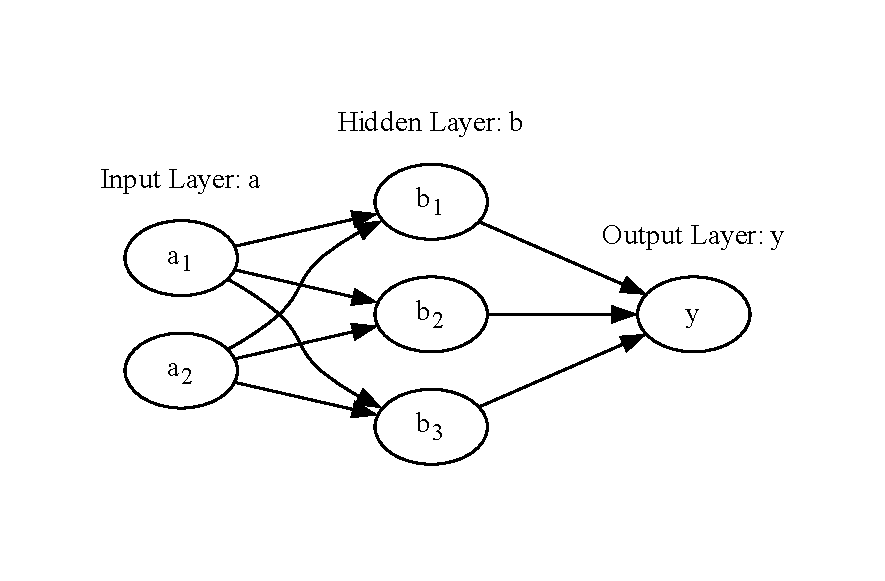
\includegraphics[width=0.5\textwidth]{graph/mlp}
  \label{fig:mlp} 
\end{figure}

Each node in b in the \ac{MLP} as seen in \figureref{fig:mlp} is calculated like the node y in \figureref{fig:perceptron}. That also means that every node combination between the layers has a weight. Such a combination of layers is called a fully connected layer. When there is a lot of correlation between all the nodes, then such a fully connected layer is useful as it is also fully utilized. However particularly when the nodes of the input layer represent the pixels of an image and the task is some form of recognition of objects in the image, most connections are not well utilized, since pixels that are further away from each other tend to have no meaningful connection \cite{aghdam2017guide}.

Convolutional layers work like a kernel based image filter but make the kernel trainable instead of static. This has the advantage that each convolutional neuron only processes data from its receptive field instead of the whole image. The receptive field of a neuron refers to the area of pixels in the source image that the data the neuron gets is dependent on. Using just one convolutional layer means that the nodes in the result are just dependent on an area in the source image as big as the kernel of that convolution. Therefore \acp{CNN} tend to have many layers to be able to recognize larger shapes in the image. The resulting data of a convolutional layer is also called a feature map. 

\section{Shapely}

Shapely is a popular Python package for computational geometry. It provides a wide range of geometric objects and operations for working with planar geometric shapes, such as points, lines and polygons. Shapely is widely used in various domains, including geographic information systems (GIS), spatial data analysis, and computer graphics.

\section{Open CV}

\ac{OpenCV} is an open-source computer vision and machine learning software library designed for various computer vision tasks such as image processing, object detection, image recognition, and more. It was originally developed by Intel and later maintained by Willow Garage and Itseez. \ac{OpenCV} is written in C++ and has interfaces for C++, Python, and other programming languages, making it widely accessible and used in both academia and industry.

\subsection{Classic ArUco Detection}



\section{Albumentations}

\section{Pytorch}

\section{HyperOpt}

\section{mAP Scores}

\subsection{Pascal Voc 2007}

\subsection{Pascal Voc 2010}

\subsection{COCO}

\chapter{Related Work}
\label{chap:relatedw}

\section{ArUco Marker Detection}

\section{Training Image Augmentations}

\section{Classic Detection Approaches?}

\chapter{Networks}
\label{chap:netw}

\section{Yolov5}

\section{Yolov8}

\section{YolovNAS}

\section{MobileNetV2}

\section{ViTs}

\chapter{Implementation}
\label{chap:implement}

\section{Used Hardware}

\section{Automated Annotations}

\section{Software Architecture}

\section{Augmentations}

\section{Synthetic Data}

\section{Plotting}

\section{Automated Evaluation of Multiple Ensemble Trainings}

\section{Hyperparameter Optimization}

\section{Point Detection}

\chapter{Evaluation}
\label{chap:eval}

\section{Test Data}

\section{Human Testing}

\section{Augmenting from Zero}

\section{Augmenting from Optimum}

\section{Discussion}

%\subsection{Confusion Matrix in Object Detection}

\chapter{Conclusion}
\label{chap:conclusion}

\section{Summary}

\section{Future Work}

\subsection{Deploying on Mobile}

\subsection{Tracking}

\chapter{Appendix}

\section{List of Abbreviations}

\begin{acronym}
% From bachelor thesis
\acro{GUI}{Graphical User Interface}
\acro{UI}{User Interface}
\acro{JSON}{JavaScript Object Notation}
\acro{SVG}{Scalable Vector Graphics}
\acro{LMB}{left mouse button}
\acro{AABB}{Axis Aligned Bounding Box}
\acroplural{AABB}{Axis Aligned Bounding Boxes}
\acro{HTML}{Hypertext Markup Language}
\acro{GIMP}{GNU Image Manipulation Program}

% From Fabio
\acro{POC}{Point-of-care}
\acro{POCT}{Point-of-care Testing Device}
\acro{IBE}{ion beam etching}
\acro{PCS}{Photonic Crystal Slab}

% From master thesis
\acro{ArUco}{Augmented Reality University of Cordoba}
\acro{GPU}{Graphics Processing Unit}
\acro{ANN}{artificial neural network}
\acro{NN}{neural network}
\acro{MLP}{multilayer feedforward network}
\acro{CNN}{convolutional neural network}
\acro{OpenCV}{Open Source Computer Vision Library}

\end{acronym}

\section{User Evaluation Files}


\backmatter
\tocbibliography

\end{document}